\documentclass[a4paper]{kulakarticle}

\usepackage[utf8]{inputenc}
\usepackage[dutch]{babel}
\usepackage{titling}
\title{Kost van een Airbnb-verblijf}
\author{Project statistiek}
\date{Academiejaar 2022 -- 2023}
\address{
	Louis Vandenbruwaene\\
	Jasper Denorme\\
	Dieter Demunck}
\usepackage{graphicx,flafter,framed,caption}
\usepackage{cprotect}
\usepackage{amsfonts,amssymb,amsmath,textcomp,eurosym,wasysym}
\usepackage{listings}
\usepackage{siunitx}
\sisetup{output-decimal-marker={,}}
\usepackage{enumitem}
\usepackage{multicol}
\usepackage{caption}
\usepackage{tabularx,array}
\usepackage{times}
\usepackage{textcomp}
\newcommand{\rood}[1]{\textcolor{red}{#1}}

\begin{document}
	\maketitle
	\section*{Inleiding}
	Airbnb is een online platform (\href{https://www.airbnb.com}{\texttt{www.airbnb.com}}) waarop reizigers een kort verblijf kunnen boeken in een accommodatie (bv. een kamer, een huis, een woonboot, …) die door particulieren wordt verhuurd. Airbnb werd opgericht in 2008 en is ondertussen een erg populair alternatief geworden voor de traditionele hotels. \\
	
	Dit onderzoek focust op de totale kostprijs voor het huren van een Airbnb-verblijf in Amsterdam voor twee personen gedurende een weekend (vrijdag tot zondag). Er wordt nagegaan met welke factoren deze kostprijs samenhangt en in welke mate de kost daarmee kan worden voorspeld. Hierbij wordt er gebruik gemaakt van een aantal veranderlijken verzameld in het kader van een onderzoeksproject uitgevoerd door Kristóf Gyódi en Łukasz Nawaro. Het gaat enerzijds over kenmerken van het verblijf en tevredenheid van eerdere gasten volgens de gegevens van Airbnb, anderzijds over de ligging van het verblijf ten opzichte van het stadscentrum, bezienswaardigheden en restaurants, telkens rekening houdend met de populariteit, zoals gerapporteerd door TripAdvisor.\\
	
	Tabel \ref{beschrijving} beschrijft de variabelen en tabellen \ref{uitreksel}, \ref{capacity tabel} en \ref{bedrooms tabel} geven enkele basisstatistieken weer van de veranderlijken, die gebruikt worden in het onderzoek. \\\\

\begin{table}[h]
	\centering
	\begin{tabular}{c|p{10cm}}
		\raggedright
		Naam & Beschrijving\\
		\hline
		realSum & Som van alle kosten voor 2 personen in euro\\ 
		room & Soort verblijf (volledige woning, afzonderlijke kamer, gedeelde kamer) \\ 
		capacity & Maximaal aantal gasten \\
		bedrooms & Aantal beschikbare slaapkamers in het verblijf \\
		dist & Afstand tot het stadscentrum (km) \\
		metro & Afstand tot dichtstbijzijnde metro-halte (km)\\
		attr & Attractiescore, nabijheid van bezienswaardigheden (op 10)\\
		rest & Restaurantscore, nabijheid van restaurants (op 10)\\ 
		host & Type verhuurder (enige beschikbare woning, 2 tot 4 beschikbare woningen, meer dan 4 beschikbare woningen) \\ 
		cleanliness & Modale score voor netheid van het verblijf volgens gasten (op 10) \\
		satisfaction & Tevredenheid van de gasten (op 10)\\
		
	\end{tabular}
	\caption{Beschrijving van de gebruikte veranderlijken.}
	\label{beschrijving}
\end{table}
\begin{table}[h]
	\centering
	\begin{tabular}{| l| l| l|  p{5cm} |}
		\hline
		Type waarde & Gemiddelde $\pm$ standaardfout  & Bereik & Algemene vorm\\  [1ex]
		\hline\hline
		Kost & €$(6 \pm 4) \cdot 10^{2} $ & $[165.9129, 8130.6681]$  &  zeer rechtsscheef\\    [0.5ex]
		\hline
		Stadscentrumafstand & $3 \pm 2$ km  & $[0.01504452, 11.19593222]$ & zeer rechtsscheef \\  [0.5ex]
		\hline
		Metroafstand & $1.1 \pm 0.8$ km & $[0.03651741, 4.41190504]$ & zeer rechtsscheef \\ [0.5ex]
		\hline
		Attractiescore & $2.1 \pm 0.9$ & $[1, 10]$  & rechtsscheef \\  [0.5ex]
		\hline
		Restaurantscore & $3 \pm 2$ & $[1, 10]$ & benaderend lognormaal met zware staarten \\ [0.5ex]
		\hline
		Netheidsscore & $9.5 \pm 0.8$ & $[2, 10]$ & benaderend exponentieel  \\ [0.5ex]
		\hline
	\end{tabular}
	\caption{Basisstatistieken van de gebruikte veranderlijken.}
	\label{uitreksel}
\end{table}

\begin{table}[h]
	\centering
	\begin{tabular}{|l|c|c|c|c|r|}
		\hline
		Max. aantal gasten&2&3&4&5&6\\[0.5ex]
		\hline
		Aantal verblijven&591&60 &301  &10  &15 \\[0.5ex]
		\hline
	\end{tabular}
	\caption{Aantal verblijven per maximaal aantal gasten.}
	\label{capacity tabel}
\end{table}

\begin{table}[h]
	\centering
	\begin{tabular}{|l|c|c|c|c|c|r|}
		\hline
		Aantal beschikbare slaapkamers&0&1&2&3&4&5\\[0.5ex]
		\hline
		Aantal verblijven&63 &636 &210   &57     &9     &2  \\[0.5ex]
		\hline
	\end{tabular}
	\caption{Aantal verblijven per het aantal slaapkamers.}
	\label{bedrooms tabel}
\end{table}


	
	\section{Methode}
	
	\subsection{Kenmerken van de steekproef}
	Om te testen of de gemiddelde kost veranderd is tegenover 2019, maken we gebruik van een student t-test voor één gemiddelde. We mogen deze gebruiken, want de dataset voldoet aan de centrale limietstelling (n = 977). Om na te gaan of het aandeel particuliere verhuurders groter is dan het aantal professionele verhuurders, maken we gebruik van een $z$-test voor één proportie.\\
	Via een $\chi^2_{3}$-test gaan we na of het aantal beschikbare kamers Poisson verdeeld is. Dit deden we nadat we de kolommen voor vier en vijf slaapkamers hebben samengevoegd om aan de Cochranregel te voldoen.
	
	\subsection{Gemiddelde kost}
	
	Hier zal onderzocht worden of de totale prijs van een verblijf voor twee personen afhankelijk is van bepaalde andere variabelen, namelijk of de netheidsscore maximaal is of niet, de eigenaar een particuliere verhuurder is of niet, en of al dan niet de volledig woning verhuurd wordt.
	Bij elke deelvraag werd eerst de normaliteit van de twee categorieën getest, aan de hand van de Shapiro-Wilk-test. We mogen deze test gebruiken aangezien voor elke variabele het aantal groot genoeg is (zie tabel \ref{tab:intermediary_results_gemiddelde_kost}). Hierna wordt een Student t-test voor twee gemiddelden bij verschillende varianties uitgevoerd, dit ook voor alle drie de deelvragen. Deze laatste test mag uitgevoerd worden, omdat de centrale limietstelling (CLS) voldaan is.

	\subsection{Associatie met de verschillende veranderlijken}
	
	Verder wordt de associatie tussen de kost van een verblijf en de andere gegevens onderzocht. Aangezien de kost (\verb|realSum|) niet normaal verdeeld is (zie figuur \ref{fig:qqplotvrealsum}) en er zelden samenvallende waarden voorkomen, wordt de associatie tussen de kost en de continue variabelen getest aan de hand van de Spearman-correlatietest. Om de afhankelijkheid met de discrete en kwalitatieve variabelen te bepalen, wordt een $\chi ^2$-test gebruikt. Hiervoor wordt de variabele de kost gediscretiseerd, door deze op te delen in zijn vier kwantielen. Ook de discrete en kwalitatieve variabele worden samengevoegd om aan de Cochranregel te voldoen. Enkel de waarden voor de types verhuurders blijft onveranderd. De opdelingen zijn te vinden in tabel \ref{tab:grenzen}. \\\\
	
	\begin{figure}
		\centering
		\includegraphics[width=0.7\linewidth]{Figuren/qqplotvrealSum}
		\caption{Kwantielplot van \textit{realSum}.}
		\label{fig:qqplotvrealsum}
	\end{figure}

	\begin{table}[h]
		\centering
			\begin{tabular}{c|c}
			\centering
			naam& opdelende grenzen\\
			\hline
			\textbf{cleanliness} & $ 0 $ - $ 7.5 $ - $ 8.5$ - $ 9.5 $ - $ 10.5$ \\
			\textbf{capacity}& $-0.5$ - $2.5$ - $3.5$ - $4.5$ - $6.5$\\
			\textbf{bedrooms}& $-0.5$ - $0.5$ - $1.5$ - $2.5$ - $6$\\
			\textbf{room} & $0.5$ - $1.5$ - $3.5$\\
			\end{tabular}
			\caption{De grenzen, die de gegevens opdelen zodat aan de Cochran-regel voldaan is.}
			\label{tab:grenzen}
	\end{table}
	\subsection{Verklaren van de kost}
	
	We zullen hier trachten de kost te verklaren aan de hand van de andere veranderlijken. Dit gebeurt met een lineair regressiemodel. Eerst wordt het model gemaakt enkel op basis van de attractiescore. Er wordt ook bestudeerd of een model gebaseerd op de $log_{10}$-transformatie van de attractiescore en van de kost een beter resultaat geeft, aangezien deze variabelen allebei rechtsscheef verdeeld zijn: skewness \verb|attr| $=2,454883$ ; skewness \verb|realSum| $=6.496029$.\\
	Daarna wordt er via achterwaartse regressie een meervoudig regressiemodel gezocht, waar we alle continue variabelen voor gebruiken en ook gebruik maken van  $log_{10}$-transformaties. Ten slotte wordt nog bestudeerd of het verhuren van de volledige woning of slechts een deel ervan een significante invloed heeft op het model. Voor alle modellen wordt de kwaliteit ook onderzocht. Dit doen we aan de hand van ingebouwde functies in R.
	\section{Resultaten}
	
	\subsection{Kenmerken van de steekproef}
	De gemiddelde kost in de steekproef is 604 euro, terwijl deze  620 euro was in 2019. Het verschil van 16 euro is niet significant ($t_{976}$ = -1.1, p = 0.29). We komen uit dat $p \approx 0$ voor onze test op het aandeel van particuliere vs. professionele verhuurders. Dit is logisch, omdat ten opzichte van het totale aantal: $977$ het absolute verschil $295$ is.\\\\
	Bij de $\chi$-kwadraat test voor onze Poisson-verdeling bekomen we $\chi^2 = 424.77$ en $p \approx 0$, een zeer lage p-waarde. Deze twee zeer lage p-waarden wijzen op een aan zekerheid grenzende waarschijnlijkheid dat er een significant verschil is tussen zowel de verschillende soorten verhuurders, als tussen de theoretische Poisson-verdeling en de steekproef.
	
	\subsection{Gemiddelde kost}
	 Uit de resultaten van de Shapiro-Wilk-testen, te zien in tabel \ref{tab:intermediary_results_gemiddelde_kost}, volgt ook dat we met aan zekerheid grenzende waarschijnlijkheid kunnen veronderstellen dat geen enkele categorie normaal verdeeld is.
	
	Uit de resultaten van de t-testen bij verschillende varianties in tabel \ref{tab:end_results_gemiddelde_kost}, zien we een zeer lage p-waarde voor de gemiddelde kost van het verhuren van de volledige woning of niet. De gemiddeldes, respectievelijk 539 euro en 355 euro, hebben een verschil van ongeveer 185 euro. We merken ook dat er een redelijke aanwijzing is dat het aantal verblijven dat een gastheer verhuurt een verschil zou betekenen in prijs. Hierbij zijn verblijven bij gastheren met meerdere woningen gemiddeld ongeveer €52 goedkoper.
	De p-waarde bij het onderzoeken van de netheidsscore ligt net onder de verwerpingsgrens. Dit kan toeval zijn, maar het zou ook een aanwijzing kunnen zijn voor een werkelijk verschil in prijs, waarbij verblijven onder de maximum netheidsscore gemiddeld ongeveer €35 goedkoper zouden zijn.
	
	\begin{table}
		\caption{Aantal datapunten, gemiddelde, en p-waarde van de Shapiro-Wilk-test (uitgevoerd op deze datapunten) van de kost voor een verblijf van 2 personen, gefilterd op bepaalde gegevens.}
		\label{tab:intermediary_results_gemiddelde_kost}
		\begin{tabular}{|l*{3}{|c}|}
			\hline
			Kost voor 2 personen bij ...        & Aantal observaties & Gemiddelde prijs & Shapiro-Wilk-test p-waarde \\ \hline
			\hline
			Maximumscore netheid                & 376    & $457.1111$ & $< 3 \cdot 10^{-16}$ \\ \hline
			Niet maximumscore netheid           & 215    & $422.2669$ & $ 3 \cdot 10^{-12}$ \\ \hline
			Gastheer verhuurt 1 woning          & 367    & $463.9553$ & $< 3 \cdot 10^{-16}$ \\ \hline
			Gastheer verhuurt meerdere woningen & 224    & $412.4534$ & $< 3 \cdot 10^{-16}$ \\ \hline
			Volledige woning wordt verhuurd     & 288    & $539.0370$ & $< 3 \cdot 10^{-16}$ \\ \hline
			Deel van de woning wordt verhuurd   & 303    & $354.5165$ & $< 3 \cdot 10^{-16}$ \\ \hline
		\end{tabular}
	\end{table}

	\begin{table}
		\caption{Verschil in gemiddelden, en p-waarde van de t-testen (bij verschillende varianties) op het verschil tussen twee categorieën van de kost van een verblijf voor twee personen.}
		\label{tab:end_results_gemiddelde_kost}
		\begin{tabular}{|l*{2}{|c}|}
			\hline
			Verschil in kost voor 2 personen tussen ...  & Verschil van gemiddelden
			& t-test p-waarde \\ \hline
			\hline
			
			Maximumscore voor netheid of niet                 & $34.84423$
			& $0.04$              \\ \hline
			Gastheer verhuurt 1 woning of meerdere       & $51.50189$
			& $0.003$             \\ \hline
			Gastheer verhuurt volledige woning of deel   & $184.5205$
			& $< 3 \cdot 10^{-16}$ \\ \hline
		\end{tabular}
	\end{table}
	
	\subsection{Associatie met de verschillende veranderlijken}
	
	Uit tabel \ref{continue variabelen afhankelijkheid} halen we de p-waarde bij de afhankelijkheidstest voor elke continue variabele met \verb|realSum|. We zien dat deze allemaal zeer klein zijn. De bijhorende correlatie wordt geschat door $\rho$.
	\begin{table}[h]
		\centering
		\begin{tabular}{c|c|c|c }
			naam & p-waarde & afhankelijkheid & $\rho$\\
			\hline
			\hline
			attr & $< 3 \cdot 10^{-16}$& ja& $0.4$ \\
			rest & $< 3 \cdot 10^{-16}$& ja& $0.4$ \\
			satisfaction & $2 \cdot 10^{-7}$& ja& $0.2$ \\
			metro & $9 \cdot 10^{-10}$& ja& $-0.2$ \\ 
			dist & $< 3 \cdot 10^{-16}$&ja& $-0.4$ \\
		\end{tabular}
		\caption{Afhankelijkheid van de prijs met de continue variabelen.}
		\label{continue variabelen afhankelijkheid}
	\end{table}
	In tabel \ref{discrete variabelen afhankelijkheid} zien we dat de p-waardes van onze $\chi^2$-test voor \verb|capacity|, \verb|bedrooms|, \verb|room| en \verb|host| zeer laag zijn terwijl deze voor \verb|cleanliness| eerder aan de hoge kant is. Het lijkt erop dat er geen of toch alleszins geen sterke correlatie is tussen cleanliness en \verb|realSum|.
	
	\begin{table}[h]
		\centering
		\begin{tabular}{c|c|c|c }
			naam & p-waarde & afhankelijkheid & $\chi ^2$\\
			\hline
			\hline
			capacity & $< 3 \cdot 10^{-16}$ & ja& $3.9 \cdot 10^{2}$ \\ 
			bedrooms & $< 3 \cdot 10^{-16}$ & ja& $3.7  \cdot 10^{2}$ \\
			room & $< 3 \cdot 10^{-16}$ & ja& $ 3.4 \cdot 10^{2}$ \\
			host & $ 6 \cdot 10^{-7}$ & ja& $40$ \\
			cleanliness & $0.8$ &nee& $5.6$ \\
		\end{tabular}
		\caption{Afhankelijkheid van de prijs met de discrete en kwalitatieve variabelen.}
		\label{discrete variabelen afhankelijkheid}
	\end{table}
	
	\subsection{Verklaren van de kost}
	
	Bij het uitvoeren van het eerste regressiemodel, waarbij enkel \textit{attr} in rekening gehouden wordt, bekomen we: 
    $ y = 338.93 + 126.58\cdot x$. Hier is $y$ de variabele \textit{realSum} en $x$ de variabele \textit{attr}. Laten we dit model de naam 'simpelmodel1' geven. Vervolgens wordt \textit{attr} vervangen door $log_{10}$(\textit{attr}) en \textit{realSum} door $log_{10}$(\textit{realSum}). Dit model noemen we 'simpelmodel2'. De bekomen vergelijking is dan: $ y = 2.55138 + 0.56912\cdot x$. Hier is $y = log_{10}$(\textit{realSum}) en $x = log_{10}$(\textit{attr}). De adjusted $R^2$ zijn te zien in tabel \ref{rsq}.\\
    
	Na het toepassen van achterwaartse regressie op ons naïef model, met alle continue variabelen, bekomen we het volgende model: $y = -190.900 + 75.886\cdot x_1 + 79.480\cdot x_2 -31.985\cdot x_3$. Hier is $y =$\textit{realsum}, $x_1 = $ \textit{satisfaction}, $x_2 =$ \textit{attr} en $x_3 =$ \textit{dist}. Hierbij lieten we \textit{rest} en \textit{metro} weg, omdat deze insignificant zijn ($p_{rest}$ = 0.77 en $p_{metro}$ = 0.46). De bijhorende adjusted $R^2$ is, zoals te zien in tabel \ref{rsq}, tamelijk laag. De residuen zijn gemiddeld ongeveer 0 (zie figuur \ref{fig:naiefmodel}). We zien duidelijk dat de grootteorde van de afwijking ook niet constant is, zelfs in de grote puntenwolk zien we een stijgende lijn. Kijken we naar het Q-Q-plot van de residuen (\ref{fig:naiefmodel}), dan zien we al sterk afwijkende staarten en de fit lijkt systematisch te onderschatten, te overschatten en dan weer te onderschatten. De residuen lijken dus niet normaal verdeeld te zijn. \\
	
	Tot slot combineren we alles tot 'onsmodel'. Hier nemen we zowel van  \verb*|realSum| als van  \verb*|attr| de $log_{10}$-transformatie, de voorspellende kracht van dit model is ook het hoogst. De residuen van het bekomen model gedragen zich ook al beter, ook hier lijken ze gemiddeld 0 te zijn met een bijna volledig constante afwijking. Als we naar de Q-Q-plot kijken van de residuen, zien we dat er nog wel redelijk sterk afwijkende staarten zijn, maar de residuen lijken nu wel al iets beter de normale verdeling beter te volgen.  
	
	\section{Discussie}
	
	\subsection{Kenmerken van de steekproef}
	Op basis van de steekproef lijkt er geen verandering te zijn in de kostprijs van een kamer. We kunnen ook met aan zekerheid grenzende waarschijnlijkheid dat er meer particulier verhuurders zijn, het lijkt er dus op dat er een 'strenge' regulering is in Amsterdam. We kunnen ook met zeer grote waarschijnlijkheid aannemen dat het aantal beschikbare kamers niet Poisson verdeeld is.
	
	\subsection{Gemiddelde kost}
	
	% I feel like this is maybe too much....
	Uit de gegevens merken we dat de prijs van een verblijf voor twee personen gemiddeld duurder wordt wanneer de volledige woning wordt verhuurd, wat op zich niet onwaarschijnlijk is.
	Er is ook een duidelijke aanwijzing dat verblijven met een gastheer die meerdere woningen verhuurd goedkoper zou zijn. Een mogelijke verklaring is dat deze gastheren voorraden aankopen voor meerdere verblijven, en dus mogelijks goedkoper grotere aantallen voorraden kunnen aankopen en deze dan kunnen verdelen onder hun verblijven. Een andere verklaring is dat zij mogelijks meer competitief zijn in hun prijs, aangezien dit hun hoofdinkomen zou zijn. In tegenstelling tot een gastheer die een verblijf verhuurt als bijzaak, moeten gastheren die dit professioneel doen een zekerheid hebben op huurders.
	Er is een grote onzekerheid of er een werkelijk verschil is in prijs tussen verblijven met en zonder de maximumscore voor netheid. Een mogelijke verklaring is dat gastheren zonder de maximumscore zelf niet goed inzien hoe vuil hun verblijf is in vergelijking met propere verblijven. Aangezien vele verblijven een netheidsscore tussen 8 en 10 hebben (zie figuur \ref{fig:cleanliness}), worden meeste gasten hier misschien weinig door afgeschrokken. Een verschil zou dan te verklaren kunnen zijn doordat vuile verblijven hun prijs moeten verlagen om een redelijk aantal gasten te kunnen hebben.
	
	\begin{figure}
		\centering
		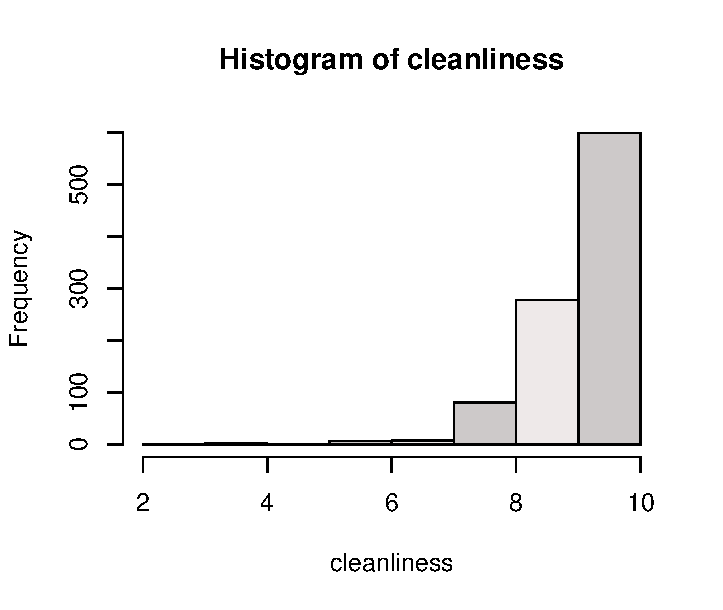
\includegraphics{Figuren/cleanliness_hist.pdf}
		\caption{Histogram van de netheidsscore.}
		\label{fig:cleanliness}
	\end{figure}
	
	\subsection{Associatie met de verschillende veranderlijken}
	
	Op basis van de steekproef zien we dat \verb*|attr|,  \verb*|rest|,  \verb*|capacity|,  \verb*|room|,  \verb*|host|,  \verb*|bedrooms| en  \verb*|satisfaction| positief gecorreleerd met de totale prijs. Waarbij de waarschijnlijkheid dat de variabelen afhankelijk zijn van elkaar groot is. Bij de continue variabelen kunnen we dit afleiden uit de $\rho$ en bij de andere kunnen we enkel kijken naar de scatterplots. \verb*|dist| en  \verb*|metro|, daarentegen, zijn negatief gecorreleerd met de totale prijs. Dit is duidelijk uit de waarde van $\rho$. Intuïtief is dit ook aanvaardbaar. Toegankelijkheid tot het stadscentrum en een metrohalte verhoogt de waarde van een verblijf. De enige variabele waarbij het lijkt dat er geen afhankelijkheid is, is  \verb*|cleanliness|.

	\begin{figure}
		\centering
		\includegraphics[width=0.49\linewidth]{Figuren/correlatievanattr}
		\includegraphics[width=0.49\linewidth]{Figuren/correlatievanrest}
		\includegraphics[width=0.49\linewidth]{Figuren/correlatievanbedrooms}
		\includegraphics[width=0.49\linewidth]{Figuren/correlatievancapacity}
		
		\caption{Scatterplots voor \textit{realSum} in functie van de meest significante veranderlijken.}
		\label{fig:correlatievanattr}
	\end{figure}




	\subsection{Verklaren van de kost}
	
	In onze zoektocht naar het optimale model, die \textit{realSum} kan voorspellen aan de hand van de andere veranderlijken in de dataset, zijn we terechtgekomen op 'onsmodel'. Met een adjusted $R^2$ van $20.06$ procent geeft dit een tamelijk slechte voorspelling van de totale prijs, maar het is al veel beter dan alle vorige modellen. De verbetering is te zien op figuur \ref{fig:naiefmodel} en \ref{fig:onsmodel}. Het uiteindelijke model heeft de volgende vorm:
	
	\begin{equation}
		\verb*|realSum| = 161.9877 \cdot (1.111806)^{ \verb*|satisfaction|} \cdot  (\verb*|attr|)^{0.402077} \cdot (0.9631125)^{ \verb*|dist|}
	\end{equation}% TODO beduidende cijfers nog
	
	We zijn tot dit model gekomen door de meest scheve veranderlijken normaler te maken met behulp van de $log_{10}$-transformatie. We hebben nog heel wat andere modellen geprobeerd, maar die hadden allen een lagere $R^2$ waarde. 
 
	\begin{figure}
		\centering
		\includegraphics[width=0.9\linewidth]{Figuren/naiefmodel}
		\caption{Residuplots voor het naïef model, ze wijzen sterk op een niet normale verdeling.}
		\label{fig:naiefmodel}
	\end{figure}
	
	
	
	\begin{table}[h]
		\centering
		\begin{tabular}{c|c|c}
			\centering
			naam van het model & adjusted $R^2$ & voorschrift van het lineair model \\
			\hline
			simpelmodel1 & $0.071$ & \textit{realSum} $\sim$ \textit{attr}\\
			simpelmodel2 &$0.18$ & $log_{10}$(\textit{realSum}) $\sim$ $log_{10}$(\textit{attr}) \\
			naïefmodel & $0.096$& \textit{realSum} $\sim$ \textit{attr}$+$\textit{satisfaction}$+$\textit{dist}\\
			onsmodel &$0.20$ & $log_{10}$(\textit{realSum}) $\sim$ $log_{10}$(\textit{attr})$+$\textit{satisfaction}$+$\textit{dist}\\
		\end{tabular}
		\caption{Enkele gebruikte modellen met hun voorschrift.}
		\label{rsq}
	\end{table} % TODO: ALLEEN LAATSTE MODEL MOET BESPROKEN WORDEN!
%==> enkel het laatste model en de andere lineaire modellen (simpelmodellen) worden besproken, ik heb deze tabel gemaakt voor de duidelijkheid en heb geen zin deze te verwijderen, anders moet een hele alinea herschreven worden.





	\begin{figure}
		\centering
		\includegraphics[width=0.9\linewidth]{Figuren/onsmodel}
		\caption{De residuplots voor 'onsmodel', de residuen volgen de normale verdeling al meer. Over het algemeen kunnen we wel nog niet besluiten dat deze normaal verdeeld zijn.}
		\label{fig:onsmodel}
	\end{figure}
	
	\begin{figure}
		\centering
		\includegraphics[width=0.9\linewidth]{Figuren/betr.attr}
		\caption{Het onderscheid tussen \textit{attr} en $log_{10}$(\textit{attr}).}
		\label{fig:betr}
	\end{figure}


	
	
	
	\section*{Besluit}
	
	
\end{document} 

